% Sources: Graph_ML/LHN_Similarity/lhn_similarity.tex and Graph_ML/Random_Walk_Similarity/random_walk_similarity.tex
\begin{notechapter}
% ---- chapter-local definitions ----
\forgetcs\bA\newcommand{\bA}{\mathbf{A}}
\forgetcs\bD\newcommand{\bD}{\mathbf{D}}
\forgetcs\bI\newcommand{\bI}{\mathbf{I}}
\forgetcs\bP\newcommand{\bP}{\mathbf{P}}
\forgetcs\bS\newcommand{\bS}{\mathbf{S}}
\forgetcs\bM\newcommand{\bM}{\mathbf{M}}
\forgetcs\bq\newcommand{\bq}{\mathbf{q}}
\forgetcs\bp\newcommand{\bp}{\mathbf{p}}
\forgetcs\be\newcommand{\be}{\mathbf{e}}
\forgetcs\bv\newcommand{\bv}{\mathbf{v}}
\forgetcs\bx\newcommand{\bx}{\mathbf{x}}
% -----------------------------------
\chapter{Node Similarity: Path Counts and Random Walks}\label{ch:node-similarity}
\chaptersubtitle{Katz, Leicht--Holme--Newman and personalized PageRank}

\begin{chapterintro}
Many graph tasks, link prediction first among them, need a number $S[u,v]$ that says how similar two nodes are. Local measures such as the number of common neighbours only look at paths of length two. The \emph{global} measures of this chapter look at paths of every length. The Katz index counts them, discounted geometrically; the Leicht--Holme--Newman (LHN) index divides each count by its expected value under a random graph with the same degrees; personalized PageRank replaces counts by the probabilities of a random walk that restarts at the source. All three are entries of the inverse of a matrix of the form $\bI - \gamma\bM$, and they differ in how they treat node degrees, which is the main theme of the chapter. We follow Hamilton (\emph{Graph Representation Learning}, 2020, Section~2.2). You will learn
\begin{itemize}[nosep]
  \item the Katz index, its closed form $(\bI - \beta\bA)^{-1} - \bI$, and its bias towards high-degree nodes;
  \item the configuration model, the expected path counts under it, and the LHN index with its closed form;
  \item random walks with restart, the personalized PageRank vector $\bq_u = (1-c)(\bI - c\bP)^{-1}\be_u$, and the similarity built from it;
  \item which degree effects each measure removes, illustrated on one small graph;
  \item (appendix) the norms and series that make the closed forms valid.
\end{itemize}
\prerequisites{adjacency and degree matrices (\cref{ch:graph-laplacians}); eigenvalues of symmetric matrices; geometric random variables.}
\end{chapterintro}

\section{A running example}\label{node-similarity:sec:running}

We compare the measures on the graph of \cref{node-similarity:fig:running}. Node $0$ is a hub of degree $6$. Nodes $1$ and $2$ have degree $2$ and the same two neighbours, $3$ and $4$, which are adjacent to each other and to the hub; nodes $5$ to $8$ are leaves of the hub. So $n = 9$, $m = 11$ and the degrees are $d = (6, 2, 2, 4, 4, 1, 1, 1, 1)$. The largest eigenvalue of $\bA$ is $\lambda_1 = 1 + \sqrt5 \approx 3.236$. Intuitively, $1$ and $2$ are structurally equivalent and should be the most similar pair involving node $1$; we will compare the pair $(1, 2)$ with the pair $(1, 0)$ (node $1$ and the hub) and the pair $(1, 5)$ (node $1$ and a leaf of the hub).

\begin{figure}[H]
\centering
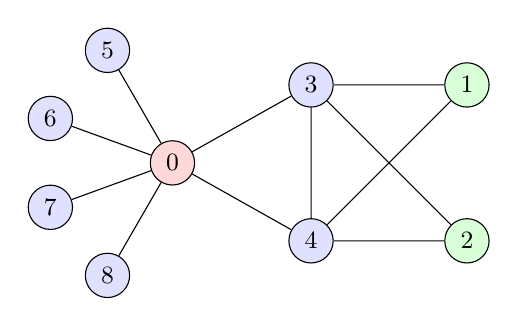
\begin{tikzpicture}[scale=1.1,
  vtx/.style={circle, draw, fill=blue!12, minimum size=16pt, inner sep=0pt, font=\small}]
  \node[vtx, fill=red!15] (0) at (0,0) {0};
  \node[vtx] (3) at (1.6,0.9) {3};
  \node[vtx] (4) at (1.6,-0.9) {4};
  \node[vtx, fill=green!15] (1) at (3.4,0.9) {1};
  \node[vtx, fill=green!15] (2) at (3.4,-0.9) {2};
  \foreach \i/\a in {5/120,6/160,7/200,8/240} \node[vtx] (\i) at (\a:1.5) {\i};
  \foreach \i in {3,4,5,6,7,8} \draw (0) -- (\i);
  \draw (3) -- (4) (1) -- (3) (1) -- (4) (2) -- (3) (2) -- (4);
\end{tikzpicture}
\caption{The running example: a hub ($0$, degree $6$) with four leaves, and two structurally equivalent nodes $1$ and $2$ of degree $2$.}
\label{node-similarity:fig:running}
\end{figure}

Recall that $\bA^i[u,v]$ is the number of walks of length $i$ from $u$ to $v$ (walks may revisit nodes; following common usage we call them paths). Here $\bA^2[1,2] = \bA^2[1,0] = 2$ (through $3$ and through $4$), $\bA^2[1,5] = 0$, and $\bA^3[u,v] = 2$ for all three pairs.

\section{Counting paths: the Katz index}

\begin{definition}[Katz index]\label{node-similarity:def:katz}
Let $\lambda_1$ be the largest eigenvalue of the adjacency matrix $\bA$ of an undirected graph. For $0 < \beta < 1/\lambda_1$, the \textbf{Katz index} of nodes $u$ and $v$ is
\begin{equation}
S_{\text{Katz}}[u,v] = \sum_{i=1}^{\infty} \beta^i \bA^i[u,v].
\label{node-similarity:eq:katz}
\end{equation}
\end{definition}

\begin{theorem}[Closed form of the Katz index]\label{node-similarity:thm:katz-closed}
For $0 < \beta < 1/\lambda_1$, $\bS_{\text{Katz}} = (\bI - \beta\bA)^{-1} - \bI$.
\end{theorem}

\begin{proof}
$\bA$ is symmetric with non-negative entries, so by the Perron--Frobenius theorem its spectral radius is $\lambda_1$, and $\beta\bA$ has spectral radius $\beta\lambda_1 < 1$. For a symmetric matrix the spectral norm equals the spectral radius, so $\norm{\beta\bA} < 1$ and the Neumann series (\cref{node-similarity:thm:neumann}) gives $(\bI - \beta\bA)^{-1} = \sum_{i\ge0}\beta^i\bA^i$. Subtract the $i = 0$ term.
\end{proof}

\begin{pitfall}[Degree bias]
High-degree nodes lie on many paths, so the Katz index favours them regardless of any special relation. In the running example, with $\beta = 0.5/\lambda_1$, $S_{\text{Katz}}[1,0] = 0.0757 > S_{\text{Katz}}[1,2] = 0.0685$: the hub beats the structurally equivalent node $2$. The two pairs have the same numbers of paths of lengths $2$ and $3$; the difference comes from longer paths, which run through the hub's many edges. The leaf pair gets $S_{\text{Katz}}[1,5] = 0.0117$.
\end{pitfall}

The question to ask is therefore not ``how many paths join $u$ and $v$?'' but ``do more paths join them than we would expect by chance, given their degrees?'' Answering it requires a model of chance.

\section{Normalizing by a null model: the LHN index}

\subsection{The configuration model}

A \emph{null model} is a random graph that represents ``nothing special going on''. Leicht, Holme and Newman (\emph{Vertex Similarity in Networks}, 2006) use one that keeps the degrees of the observed graph and randomizes everything else.

\begin{definition}[Configuration model]\label{node-similarity:def:configuration}
Given a degree sequence $(d_1, \ldots, d_n)$ with $\sum_u d_u = 2m$, the \textbf{configuration model} generates a random multigraph as follows: give each node $u$ exactly $d_u$ \emph{stubs} (half-edges), then pair the $2m$ stubs uniformly at random, each pair forming an edge.
\end{definition}

Every node of the random graph $G'$ has the same degree as in the observed graph $G$, but the wiring is random. (Self-loops and multiple edges can occur; their expected number stays bounded as $m$ grows with bounded degrees, and they are ignored below.) A simpler null model such as the Erd\H{o}s--R\'enyi graph, where every edge is present with the same probability, would make high-degree nodes look special merely for having high degree; fixing the degrees removes this effect.

\begin{pitfall}[Two adjacency matrices]
Two matrices play different roles. $\bA$ is the adjacency matrix of the \emph{observed}, fixed graph $G$; $\bA^i[u,v]$ is a number computed from the data. $\bA_{G'}$ is the adjacency matrix of a random graph $G'$ drawn from the configuration model; it is a random matrix, and
\begin{equation}
\E\bigl[\bA_{G'}^i[u,v]\bigr] = \sum_{G'} P(G')\,\bA_{G'}^i[u,v],
\label{node-similarity:eq:expectation-formal}
\end{equation}
the sum running over all multigraphs the stub pairing can produce. The LHN index compares $\bA^i[u,v]$ with this expectation.
\end{pitfall}

\subsection{Expected path counts}

\begin{proposition}[Expected edge count]\label{node-similarity:prop:expected-edge}
For $u \ne v$, under the configuration model
\begin{equation}
\E\bigl[\bA_{G'}[u,v]\bigr] = \frac{d_u d_v}{2m - 1} \approx \frac{d_u d_v}{2m}.
\label{node-similarity:eq:expected-edge}
\end{equation}
\end{proposition}

\begin{proof}
Number the stubs of $u$ by $s = 1, \ldots, d_u$ and those of $v$ by $t = 1, \ldots, d_v$, and let $X_{s,t}$ be the indicator that stub $s$ is paired with stub $t$. Then $\bA_{G'}[u,v] = \sum_{s,t} X_{s,t}$. In a uniform random pairing, stub $s$ is equally likely to be paired with each of the other $2m - 1$ stubs, so $\E[X_{s,t}] = P(X_{s,t} = 1) = 1/(2m-1)$. By linearity of expectation, $\E[\bA_{G'}[u,v]] = d_ud_v/(2m-1)$.
\end{proof}

\begin{proposition}[Expected length-2 path count]\label{node-similarity:prop:expected-path2}
For $u \ne v$, up to factors $1 + O(1/m)$,
\begin{equation}
\E\bigl[\bA_{G'}^2[u,v]\bigr] \approx \frac{d_u d_v}{(2m)^2} \sum_{w \in V} d_w(d_w - 1).
\label{node-similarity:eq:expected-path2}
\end{equation}
\end{proposition}

\begin{proof}
$\bA_{G'}^2[u,v] = \sum_w \bA_{G'}[u,w]\bA_{G'}[w,v]$. A path $u - w - v$ uses a stub $s$ of $u$ paired with a stub $r$ of $w$, and a \emph{different} stub $r'$ of $w$ paired with a stub $t$ of $v$. There are $d_u\,d_w(d_w - 1)\,d_v$ choices of $(s, r, r', t)$, and each pair of pairings occurs with probability $\frac{1}{2m-1}\cdot\frac{1}{2m-3} \approx \frac{1}{(2m)^2}$ (after pairing $s$ with $r$, $2m - 2$ stubs remain). Summing over $w$ gives the claim.
\end{proof}

The factor $\sum_w d_w(d_w - 1)/(2m)$ is the mean excess degree: the expected number of further edges at the end of a randomly chosen edge. For paths of length $i\ge3$ an exact computation must track repeated nodes and correlations between pairings, and Leicht, Holme and Newman do not attempt it. They use instead the growth rate of path counts.

\subsection{Spectral approximation for long paths}

Fix a source $u$ and let $\bp_i = \bA^i\be_u$, so that $\bp_i[v] = \bA^i[u,v]$. The recurrence $\bp_i = \bA\bp_{i-1}$ says that a path of length $i$ to $v$ is a path of length $i-1$ to a neighbour $w$ of $v$ followed by the edge $(w, v)$.

\begin{example}[Path count recurrence]
On the triangle, $\bA = \bigl(\begin{smallmatrix}0&1&1\\1&0&1\\1&1&0\end{smallmatrix}\bigr)$ and $\bp_0 = (1, 0, 0)^\top$ give $\bp_1 = (0, 1, 1)^\top$ and $\bp_2 = (2, 1, 1)^\top$: two closed paths $1 \to 2 \to 1$ and $1 \to 3 \to 1$, and one path to each other node. Further, $\bp_3 = (2, 3, 3)^\top$ and $\bp_4 = (6, 5, 5)^\top$: the totals $1, 2, 4, 8, 16$ double at each step, and $\lambda_1 = 2$.
\end{example}

\begin{theorem}[Asymptotic path growth]\label{node-similarity:thm:path-growth}
Let $G$ be connected and not bipartite, with eigenvalues $\lambda_1 > \lambda_2 \ge \cdots \ge \lambda_n$ of $\bA$ and unit eigenvector $\bv_1$ for $\lambda_1$. Then $\bp_i/\lambda_1^i \to \bv_1[u]\,\bv_1$, so $\bp_i \approx \lambda_1\bp_{i-1}$ for large $i$.
\end{theorem}

\begin{proof}
Expand $\be_u = \sum_j c_j\bv_j$ in an orthonormal eigenbasis, with $c_j = \bv_j[u]$. Then $\bp_i = \sum_j c_j\lambda_j^i\bv_j$ and $\bp_i/\lambda_1^i = c_1\bv_1 + \sum_{j\ge2}c_j(\lambda_j/\lambda_1)^i\bv_j$. For a connected graph, Perron--Frobenius gives a simple $\lambda_1$ with a positive eigenvector (so $c_1 > 0$), and for a non-bipartite graph also $\abs{\lambda_j} < \lambda_1$ for $j \ge 2$. The sum therefore tends to $0$.
\end{proof}

On a bipartite graph $\lambda_n = -\lambda_1$ and the counts alternate between the two sides, so the ratio $\bp_i[v]/\bp_{i-1}[v]$ does not converge. Leicht, Holme and Newman combine the theorem with \cref{node-similarity:prop:expected-edge}: the expected number of paths of length $1$ is $d_ud_v/2m$, and each further step multiplies counts by about $\lambda_1$. This gives the heuristic
\begin{equation}
\E\bigl[\bA_{G'}^i[u,v]\bigr] \approx \frac{d_u d_v}{2m}\,\lambda_1^{\,i-1}, \qquad i \ge 1 .
\label{node-similarity:eq:expected-path-approx}
\end{equation}

\begin{remark}
\Cref{node-similarity:eq:expected-path-approx} is an approximation, not a theorem: it applies the growth rate of the \emph{observed} graph to the expected counts in the \emph{random} graph. For $i = 2$ it replaces the mean excess degree of \cref{node-similarity:prop:expected-path2} by $\lambda_1$. In the running example the mean excess degree is $\sum_w d_w(d_w-1)/2m = 60/22 \approx 2.73$, against $\lambda_1 \approx 3.24$; the approximation is of the right order, which is all the index needs.
\end{remark}

\subsection{The LHN index}

Divide each path count by its approximate expectation and weight the ratios as in the Katz index:
\[
\frac{\bA^i[u,v]}{\E[\bA_{G'}^i[u,v]]} \approx \frac{2m}{d_ud_v}\,\lambda_1^{1-i}\,\bA^i[u,v],
\qquad
S_{\text{LHN}}[u,v] = \frac{2m}{d_ud_v}\sum_{i=0}^\infty\beta^i\lambda_1^{1-i}\bA^i[u,v].
\]
The $i = 0$ term affects only the diagonal $u = v$. Some authors (and the original source of these notes) drop it and add the identity instead, which changes nothing for distinct nodes.

\begin{theorem}[Closed form of the LHN index]\label{node-similarity:thm:lhn-closed}
For $0 < \beta < 1$,
\begin{equation}
\bS_{\text{LHN}} = 2m\lambda_1\,\bD^{-1}\left(\bI - \frac{\beta}{\lambda_1}\bA\right)^{-1}\bD^{-1}.
\label{node-similarity:eq:lhn-closed}
\end{equation}
\end{theorem}

\begin{proof}
Write $\beta^i\lambda_1^{1-i} = \lambda_1(\beta/\lambda_1)^i$. The matrix $\frac{\beta}{\lambda_1}\bA$ is symmetric with spectral radius $\beta < 1$, so by the Neumann series $\sum_{i\ge0}(\frac{\beta}{\lambda_1}\bA)^i = (\bI - \frac{\beta}{\lambda_1}\bA)^{-1}$. Finally, multiplying entry $(u, v)$ by $1/(d_ud_v)$ is the same as multiplying by $\bD^{-1}$ on both sides.
\end{proof}

Note the convergence condition: $\beta < 1$, not $\beta < 1/\lambda_1$, because the powers of $\bA$ are already divided by $\lambda_1^i$. Hamilton (2020) writes \cref{node-similarity:eq:lhn-closed} with a different constant in front; a global constant does not affect rankings. Large $\beta$ (close to $1$) gives weight to long paths, small $\beta$ to short ones.

\begin{example}[LHN on the running example]
With $\beta = 0.5$, \cref{node-similarity:eq:lhn-closed} gives $S_{\text{LHN}}[1,2] = 1.219$, $S_{\text{LHN}}[1,0] = 0.449$ and $S_{\text{LHN}}[1,5] = 0.416$. The ranking is reversed compared with Katz: the hub is no longer favoured, because its paths to node $1$ are about as many as its degree predicts. With $\beta = 0.9$ the values are $14.61$, $7.05$ and $11.77$: node $2$ is still first, but the leaf $5$ now beats the hub. The factor $1/(d_ud_v)$ boosts low-degree nodes, and for $\beta$ close to $1$ long paths through the hub reach the leaf in large numbers; LHN with large $\beta$ can overcorrect.
\end{example}

\section{Random walks with restart: personalized PageRank}

\subsection{The transition matrix}

\begin{definition}[Transition matrix]\label{node-similarity:def:transition}
For a graph without isolated nodes, the \textbf{random-walk transition matrix} is
\begin{equation}
\bP = \bA\bD^{-1}, \qquad \bP[v,u] = \frac{\bA[v,u]}{d_u},
\label{node-similarity:eq:transition}
\end{equation}
the probability of moving from $u$ to $v$ in one step of a walk that leaves $u$ along a uniformly chosen edge.
\end{definition}

Each column of $\bP$ sums to $1$ ($\bP$ is \emph{column-stochastic}), and if $\bq$ is the distribution of the walker's position, $\bP\bq$ is the distribution one step later. On a connected non-bipartite graph the walk converges, from any starting point, to the stationary distribution $\pi_v = d_v/2m$ (indeed $\bP\boldsymbol\pi = \bA\bD^{-1}\bD\mathbf1/2m = \bA\mathbf1/2m = \boldsymbol\pi$). This limit does not depend on the starting node, so it carries no information about pairs. Restarts fix that.

\subsection{Personalized PageRank}

Consider a walker that, at each step, follows a random edge with probability $c$ and jumps back to the source $u$ with probability $1 - c$. If $\bq_u^{(t)}$ is the distribution of its position at time $t$, the walker is at $v$ at time $t + 1$ either because it took a step from some $w$ (probability $c\sum_w\bP[v,w]\bq_u^{(t)}[w]$) or because it restarted and $v = u$ (probability $(1-c)\be_u[v]$). Hence
\begin{equation}
\bq_u^{(t+1)} = c\bP\bq_u^{(t)} + (1-c)\be_u .
\label{node-similarity:eq:ppr-dynamics}
\end{equation}

\begin{definition}[Personalized PageRank]\label{node-similarity:def:ppr}
For a source node $u$ and damping factor $c\in(0,1)$, the \textbf{personalized PageRank vector} $\bq_u$ is the solution of
\begin{equation}
\bq_u = c\bP\bq_u + (1-c)\be_u .
\label{node-similarity:eq:ppr-recurrence}
\end{equation}
\end{definition}

\begin{proposition}[Closed form and convergence]\label{node-similarity:prop:ppr-closed}
For $c\in(0,1)$, $\bI - c\bP$ is invertible and
\begin{equation}
\bq_u = (1-c)(\bI - c\bP)^{-1}\be_u = (1-c)\sum_{k=0}^\infty c^k\bP^k\be_u .
\label{node-similarity:eq:ppr-closed}
\end{equation}
$\bq_u$ is a probability vector, and the iteration \eqref{node-similarity:eq:ppr-dynamics} converges to it from any initial distribution, with $\norm{\bq_u^{(t)} - \bq_u}_1 \le 2c^t$.
\end{proposition}

\begin{proof}
In the norm $\norm{\bM}_1 = \max_j\sum_i\abs{\bM_{ij}}$ (maximal column sum), $\norm{\bP}_1 = 1$, so $\norm{c\bP}_1 = c < 1$. The Neumann series (\cref{node-similarity:thm:neumann}) gives invertibility and the series; rearranging \eqref{node-similarity:eq:ppr-recurrence} as $(\bI - c\bP)\bq_u = (1-c)\be_u$ gives the closed form. Every $\bP^k\be_u$ is a probability vector, and the weights $(1-c)c^k$ sum to $1$, so $\bq_u$ is one too. For the iteration, subtracting \eqref{node-similarity:eq:ppr-recurrence} from \eqref{node-similarity:eq:ppr-dynamics} gives $\bq_u^{(t)} - \bq_u = (c\bP)^t(\bq_u^{(0)} - \bq_u)$, whose $1$-norm is at most $c^t\cdot2$.
\end{proof}

\begin{pitfall}[The spectral norm of $\bP$ can exceed $1$]
The proof uses the $1$-norm on purpose. Although every eigenvalue of $\bP$ has modulus at most $1$ (\cref{node-similarity:prop:eigenvalue-bound}), $\bP$ is not symmetric and its spectral norm $\norm{\bP}_2$ can be larger than $1$: for the running example, $\norm{\bP}_2 \approx 2.03$. (Take $\bx$ equal to $1$ on the leaves $5, \ldots, 8$: $\bP\bx$ puts mass $4$ on the hub, so $\norm{\bP\bx}_2 = 4 > \norm{\bx}_2 = 2$.) An argument via $\norm{c\bP}_2 < 1$ is therefore wrong; the $1$-norm, in which $\bP$ is a contraction of probability vectors, is the natural one.
\end{pitfall}

The series \eqref{node-similarity:eq:ppr-closed} says that personalized PageRank is an average of the $k$-step distributions $\bP^k\be_u$ with geometric weights $(1-c)c^k$: the walk length $K$ before the first restart is geometric, $P(K = k) = (1-c)c^k$, and $\bq_u$ is the distribution of the position after $K$ steps. Its mean is $\E[K] = \sum_k k(1-c)c^k = c/(1-c)$, using $\sum_k kc^k = c/(1-c)^2$ (differentiate the geometric series). For the classical choice $c = 0.85$ of PageRank (Page et al., \emph{The PageRank Citation Ranking: Bringing Order to the Web}, 1999) this is $5.67$ steps; counting the restart step too gives $1/(1-c) \approx 6.67$. Small $c$ keeps $\bq_u$ near $\be_u$ (only the source matters); as $c \to 1$, $\bq_u$ tends to the stationary distribution $\pi_v = d_v/2m$, which forgets the source.

\subsection{Random-walk similarity}

\begin{definition}[Random-walk similarity]\label{node-similarity:def:rw-sim}
The \textbf{random-walk similarity} of $u$ and $v$ is $S_{\text{RW}}[u,v] = \bq_u[v] + \bq_v[u]$.
\end{definition}

The sum is symmetric by construction, while $\bq_u[v]$ and $\bq_v[u]$ differ in general. On an undirected graph the difference has a simple form.

\begin{proposition}[Reversibility]\label{node-similarity:prop:reversibility}
On an undirected graph, $\bq_u[v]/d_v = \bq_v[u]/d_u$ for all $u, v$. Consequently
\[
S_{\text{RW}}[u,v] = (d_u + d_v)\,R[u,v], \qquad R[u,v] = \frac{\bq_u[v]}{d_v} = (1-c)\bigl[(\bD - c\bA)^{-1}\bigr]_{uv},
\]
where $R$ is a symmetric matrix.
\end{proposition}

\begin{proof}
$\bI - c\bA\bD^{-1} = (\bD - c\bA)\bD^{-1}$, so $(\bI - c\bP)^{-1} = \bD(\bD - c\bA)^{-1}$ and $\bq_u[v] = (1-c)[\bD(\bD - c\bA)^{-1}]_{vu} = (1-c)\,d_v\,[(\bD - c\bA)^{-1}]_{vu}$. The matrix $\bD - c\bA$ is symmetric, hence so is its inverse.
\end{proof}

So personalized PageRank divides out the degree of the \emph{source} (the walker leaves $u$ along one of $d_u$ edges) but not that of the \emph{target}: $\bq_u[v]$ is proportional to $d_v$, just as the stationary distribution is. Hubs collect probability.

\begin{example}[Personalized PageRank on the running example]
With $c = 0.85$: $\bq_1[2] = \bq_2[1] = 0.0874$, so $S_{\text{RW}}[1,2] = 0.175$; $\bq_1[0] = 0.169$ and $\bq_0[1] = 0.056$, so $S_{\text{RW}}[1,0] = 0.225$; and $S_{\text{RW}}[1,5] = 0.072$. As for Katz, the hub comes first. The degree-free part $R[u,v]$ of \cref{node-similarity:prop:reversibility} gives $R[1,2] = 0.0437 > R[1,0] = 0.0281 > R[1,5] = 0.0239$, the same order as LHN with $\beta = 0.5$. The two asymmetric scores also obey the proposition: $0.169/6 = 0.056/2 = 0.0281$.
\end{example}

\section{Comparison}

\begin{center}
\small
\begin{tabular}{@{}llll@{}}
\toprule
 & \textbf{Katz} & \textbf{LHN} & \textbf{Personalized PageRank} \\
\midrule
Basic quantity & path counts $\bA^i[u,v]$ & counts over expected counts & walk probabilities $\bP^k[v,u]$ \\
Weights & $\beta^i$ & $\beta^i$ & $(1-c)c^k$ \\
Closed form & $(\bI - \beta\bA)^{-1} - \bI$ & $2m\lambda_1\bD^{-1}(\bI - \tfrac{\beta}{\lambda_1}\bA)^{-1}\bD^{-1}$ & $(1-c)(\bI - c\bP)^{-1}$ \\
Convergence & $\beta < 1/\lambda_1$ & $\beta < 1$ & $c < 1$ \\
Degree effect & favours hubs & divides by $d_ud_v$ & divides by $d_u$, keeps $d_v$ \\
\bottomrule
\end{tabular}
\end{center}

\begin{keyidea}
All three measures are resolvents, inverses of $\bI - \gamma\bM$ for a suitably normalized $\bM$, and hence weighted sums over paths of all lengths. They differ in how they normalize by degree: Katz not at all, personalized PageRank by the degree of the node the walk leaves, and LHN by the degrees of both endpoints together with the growth rate $\lambda_1$.
\end{keyidea}

\paragraph{Computation.} Each measure requires a linear solve per source node: $O(n^3)$ for all pairs by dense inversion, and for one source a sparse iterative solve, power iteration (which converges at rate $c$ for personalized PageRank by \cref{node-similarity:prop:ppr-closed}), or a local ``push'' algorithm that only touches nodes with non-negligible scores. LHN also needs $\lambda_1$, which power iteration on $\bA$ provides in $O(\abs{E})$ per iteration. The choice of measure depends on whether degree is informative: Katz when popularity itself predicts links, LHN or the degree-normalized random-walk score when one looks for structural similarity between nodes of different degrees.

\begin{chaptersummary}
\begin{itemize}
\item The Katz index $\sum_{i\ge1}\beta^i\bA^i = (\bI - \beta\bA)^{-1} - \bI$ ($\beta < 1/\lambda_1$) counts paths of all lengths with geometric weights; it favours high-degree nodes.
\item Under the configuration model (random pairing of stubs, degrees fixed), $\E[\bA_{G'}[u,v]] = d_ud_v/(2m-1)$ and $\E[\bA_{G'}^2[u,v]] \approx d_ud_v\sum_wd_w(d_w-1)/(2m)^2$; longer paths are approximated by $d_ud_v\lambda_1^{i-1}/2m$, using the growth rate $\lambda_1$ of path counts on a connected non-bipartite graph.
\item The LHN index divides observed by expected counts; its closed form is $2m\lambda_1\bD^{-1}(\bI - \frac{\beta}{\lambda_1}\bA)^{-1}\bD^{-1}$, convergent for $\beta < 1$. It removes the hub bias, and can overcorrect towards low-degree nodes for $\beta$ near $1$.
\item Personalized PageRank $\bq_u = (1-c)(\bI - c\bP)^{-1}\be_u$, with $\bP = \bA\bD^{-1}$, is the position of a random walk after a geometric number of steps. The Neumann series converges in the $1$-norm, in which $\norm{\bP}_1 = 1$; the spectral norm of $\bP$ can exceed $1$.
\item On undirected graphs $\bq_u[v]/d_v$ is symmetric in $u, v$: personalized PageRank normalizes the source degree but keeps the target degree, so $S_{\text{RW}} = \bq_u[v] + \bq_v[u]$ still favours hubs.
\end{itemize}
\end{chaptersummary}

\chapterappendix

\section{Norms, eigenvalues and the Neumann series}

\begin{definition}[Induced matrix norms]\label{node-similarity:def:norms}
For a square matrix $\bM$, the norm induced by a vector norm $\norm\cdot$ is $\norm{\bM} = \max_{\bx\ne0}\norm{\bM\bx}/\norm{\bx}$. For the $1$-norm this is the maximal column sum, $\norm{\bM}_1 = \max_j\sum_i\abs{\bM_{ij}}$; for the Euclidean norm it is the largest singular value $\sigma_{\max}(\bM)$, which equals $\max_i\abs{\lambda_i}$ when $\bM$ is symmetric. Induced norms are submultiplicative: $\norm{\bM\bM'} \le \norm{\bM}\,\norm{\bM'}$.
\end{definition}

The column-sum formula follows from $\norm{\bM\bx}_1 \le \sum_i\sum_j\abs{\bM_{ij}}\abs{x_j} \le \max_j(\sum_i\abs{\bM_{ij}})\norm{\bx}_1$, with equality for $\bx = \be_j$ at the maximizing column. In particular a column-stochastic $\bP$ has $\norm{\bP}_1 = 1$.

\begin{proposition}[Eigenvalues of stochastic matrices]\label{node-similarity:prop:eigenvalue-bound}
Every eigenvalue $\lambda$ of a column-stochastic matrix $\bP$ satisfies $\abs{\lambda} \le 1$.
\end{proposition}

\begin{proof}
$\bP^\top$ has the same eigenvalues and its rows sum to $1$. If $\bP^\top\bx = \lambda\bx$ and $\abs{x_i} = \max_j\abs{x_j} > 0$, then $\abs\lambda\abs{x_i} = \abs{\sum_j\bP_{ji}x_j} \le \sum_j\bP_{ji}\abs{x_i} = \abs{x_i}$. (This is the Gershgorin argument applied to columns.)
\end{proof}

\begin{theorem}[Neumann series]\label{node-similarity:thm:neumann}
If $\norm{\bM} < 1$ in some induced norm, then $\bI - \bM$ is invertible and $(\bI - \bM)^{-1} = \sum_{k=0}^\infty\bM^k$, the series converging absolutely. The same holds when $\bM$ is symmetric with spectral radius less than $1$.
\end{theorem}

\begin{proof}
Since $\norm{\bM^k} \le \norm{\bM}^k$, the series $\sum_k\norm{\bM^k}$ is dominated by a convergent geometric series, so $\bS = \sum_k\bM^k$ converges. Its partial sums $\bS_K$ satisfy $(\bI - \bM)\bS_K = \bS_K(\bI - \bM) = \bI - \bM^{K+1} \to \bI$, so $\bS$ is a two-sided inverse of $\bI - \bM$. For symmetric $\bM$, the spectral norm equals the spectral radius, which reduces the second statement to the first.
\end{proof}

The theorem is the matrix version of $1/(1-x) = \sum_kx^k$ for $\abs x < 1$. Applied to $\bM = c\bP$ in the $1$-norm it gives \cref{node-similarity:prop:ppr-closed}; applied to the symmetric matrices $\beta\bA$ and $\frac{\beta}{\lambda_1}\bA$ it gives the Katz and LHN closed forms.

\section*{Further reading}
\addcontentsline{toc}{section}{Further reading}
Hamilton (\emph{Graph Representation Learning}, 2020, Chapter~2) presents these measures as ``global overlap'' statistics alongside local ones such as common neighbours and the Jaccard index. The LHN index is from Leicht, Holme and Newman (\emph{Vertex Similarity in Networks}, Physical Review E, 2006); the Katz index goes back to Katz (\emph{A New Status Index Derived from Sociometric Analysis}, 1953); PageRank to Page, Brin, Motwani and Winograd (1999). Lü and Zhou (\emph{Link Prediction in Complex Networks: A Survey}, 2011) compare these and many other similarity indices on real networks, and Leskovec, Rajaraman and Ullman (\emph{Mining of Massive Datasets}, 2020) treat the computation of PageRank at scale.

\section*{Exercises}
\addcontentsline{toc}{section}{Exercises}

\begin{exercise}\label{node-similarity:exr:1}
On the path $1 - 2 - 3$, compute $\lambda_1$ and the Katz index $S_{\text{Katz}}[1,3]$ in closed form as a function of $\beta$. Check it against the first terms of the series.
\hint{$\bA^{2k}[1,3] = 2^{k-1}$ for $k \ge 1$ and odd powers vanish.}
\solutionlink{node-similarity:exr:1}
\end{exercise}

\begin{exercise}\label{node-similarity:exr:2}
Under the configuration model with degree sequence $(2, 2, 1, 1)$, enumerate the possible pairings of the six stubs, and compute $\E[\bA_{G'}[1,2]]$ exactly (nodes $1, 2$ have degree $2$). Compare with $d_1d_2/(2m-1)$ and $d_1d_2/2m$.
\hint{There are $5\cdot3\cdot1 = 15$ pairings, all equally likely.}
\solutionlink{node-similarity:exr:2}
\end{exercise}

\begin{exercise}\label{node-similarity:exr:3}
On the star with centre $0$ and leaves $1, 2, 3$, compute the personalized PageRank vector $\bq_0$ for general $c$, and $\bq_1[0]$. Verify \cref{node-similarity:prop:reversibility}.
\hint{By symmetry $\bq_0 = (a, b, b, b)$; write the two equations of \eqref{node-similarity:eq:ppr-recurrence}.}
\solutionlink{node-similarity:exr:3}
\end{exercise}

\begin{exercise}\label{node-similarity:exr:4}
Show that for a $k$-regular connected graph (all degrees $k$) the three measures induce the same ranking of pairs: $S_{\text{Katz}}$ with parameter $\beta$, $S_{\text{LHN}}$ with parameter $\beta k$, and $S_{\text{RW}}$ with $c = \beta k$ are, off the diagonal, positive multiples of one another.
\solutionlink{node-similarity:exr:4}
\end{exercise}

\begin{exercise}\label{node-similarity:exr:5}
Show that $\norm{\bP}_2 \ge \sqrt{\ell}$ for the transition matrix of a star with $\ell$ leaves, so that no bound $\norm{\bP}_2 \le 1$ can hold for general graphs.
\solutionlink{node-similarity:exr:5}
\end{exercise}
\end{notechapter}
